%===================================================================================
\chapter{Code Organization}\label{s:organization}
%===================================================================================

%----------------------------------
\section{SUNDIALS organization}\label{ss:sun_org}
%----------------------------------
% This is a shared SUNDIALS TEX file with description of
% the SUNDIALS organization
%
The family of solvers referred to as {\sundials} consists of the solvers
{\cvode} (for ODE systems), {\kinsol} (for nonlinear algebraic
systems), and {\ida} (for differential-algebraic systems).  In addition,
{\sundials} also includes variants of {\cvode} and {\ida} with sensitivity analysis 
capabilities (using either forward or adjoint methods): {\cvodes} and {\idas},
respectively.

The various solvers of this family share many subordinate modules.
For this reason, it is organized as a family, with a directory
structure that exploits that sharing (see Fig. \ref{f:sunorg}).
\begin{figure}
\subfigure[High-level diagram]
{\centerline{\psfig{figure=sunorg1.eps,width=\textwidth}}}
\subfigure[Directory structure of the source tree]
{\centerline{\psfig{figure=sunorg2.eps,width=\textwidth}}}
\caption {Organization of the SUNDIALS suite}\label{f:sunorg}
\end{figure}
The following is a list of the solver packages presently available:
\begin{itemize}

\item {\cvode},  
  a solver for stiff and nonstiff ODEs $dy/dt = f(t,y)$;

\item {\cvodes},
  a solver for stiff and nonstiff ODEs
  with sensitivity analysis capabilities;

\item {\ida},
  a solver for differential-algebraic systems $F(t,y,y^\prime) = 0$;

\item {\idas},
  a solver for differential-algebraic systems
  with sensitivity analysis capabilities;

\item {\kinsol}, 
  a solver for nonlinear algebraic systems $F(u) = 0$.

\end{itemize}


%----------------------------------
\section{KINSOL organization}\label{ss:kinsol_org}
%----------------------------------

\index{KINSOL@{\kinsol}!package structure}
The {\kinsol} package is written in the ANSI {\CC} language. This section
summarizes the basic structure of the package, although knowledge
of this structure is not necessary for its use.

The overall organization of the {\kinsol} package is shown in Figure
\ref{f:kinorg}.
\begin{figure}[htb]
{\centerline{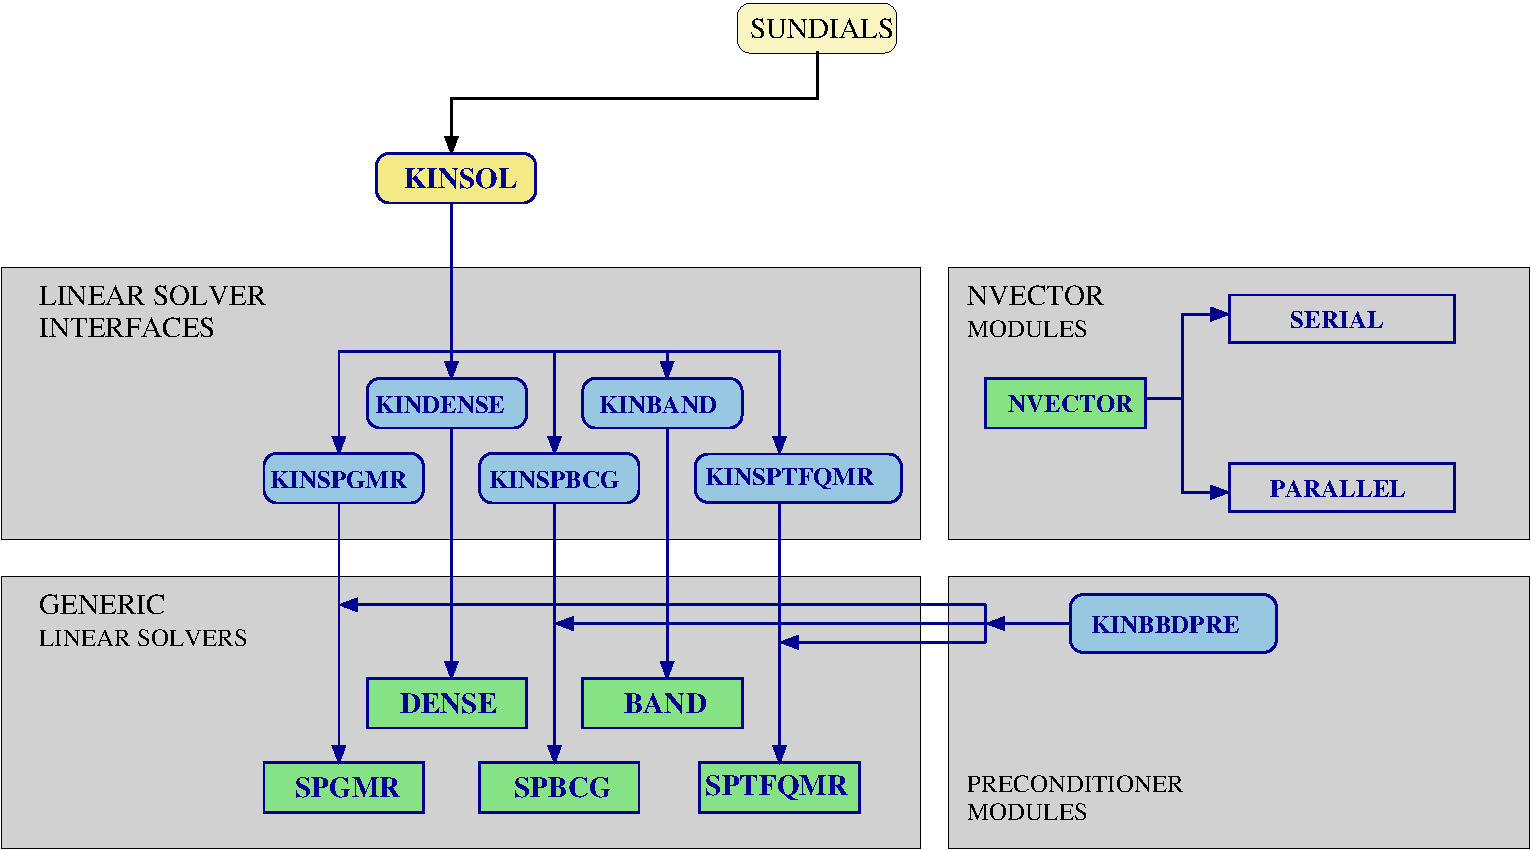
\includegraphics[width=\textwidth]{kinorg}}}
\caption [Overall structure diagram of the KINSOL package]
{Overall structure diagram of the {\kinsol} package.
  Modules specific to {\kinsol} are distinguished by rounded boxes, while
  generic solver and auxiliary modules are in rectangular boxes.
  Grayed boxes refer to the encompassing {\sundials} structure.
  Note also that the LAPACK, {\klu} and {\superlumt} support is
  through interfaces to external packages. 
  Users will need to download and compile those packages independently.}
\label{f:kinorg}
\end{figure}
The central solver module, implemented in the files
\id{kinsol.h}, \id{kinsol\_impl.h} and \id{kinsol.c}, deals with the solution
of a nonlinear algebraic system using either an Inexact Newton method or a
line search method for the global strategy. Although this module contains logic
for the Newton iteration, it has no knowledge of the method used to solve the
linear systems that arise. For any given user problem, one of the linear system
solve rinterfaces is specified, and is then invoked as needed.

\index{KINSOL@{\kinsol} linear solver interfaces|(}
At present, the package includes two linear solver interfaces.  The
{\em direct} linear solver interface, {\kindls}, supports {\sunlinsol}
implementations with type \id{SUNLINSOL\_DIRECT} (see Chapter
\ref{s:sunlinsol}).  These linear solvers utilize direct methods for
the solution of linear systems stored using one of the {\sundials} generic
{\sunmatrix} implementations (dense, banded or sparse; see
Chapter \ref{s:sunmatrix}).  
The {\em spils} linear solver interface, {\kinspils}, supports
{\sunlinsol} implementations with type \id{SUNLINSOL\_ITERATIVE}
(see Chapter \ref{s:sunlinsol}).  These linear solvers utilize scaled
preconditioned iterative methods.  It is assumed that these methods
are implemented in a ``matrix-free'' manner, wherein only the action
of the matrix-vector product is required.  Since {\kinsol} can
operate on any valid {\sunlinsol} implementation of
\id{SUNLINSOL\_DIRECT} or \id{SUNLINSOL\_ITERATIVE} types, the set of
linear solver modules available to {\kinsol} will expand as new
{\sunlinsol} modules are developed.

Within the {\kindls} interface, the package includes algorithms for the
approximation of dense or banded Jacobians through difference 
quotients, but the user also has the option of supplying the Jacobian
(or an approximation to it) directly.  This user-supplied 
routine is required when using sparse Jacobian matrices, since
standard difference quotient approximations do not leverage the
inherent sparsity of the problem.

Within the {\kinspils} interface, the package includes an algorithm for
the approximation by difference quotients of the product between the Jacobian
matrix and a vector. Again,
the user has the option of providing routines for this operation, in
two phases: setup (preprocessing of Jacobian data) and multiplication.
For preconditioned iterative methods, \index{preconditioning!setup and solve phases} 
the preconditioning must be supplied by the user, again in two phases: 
setup and solve.  While\index{preconditioning!advice on} there is no
default choice of preconditioner analogous to the difference-quotient
approximation in the direct case, the references
\cite{BrHi:89,Byr:92}, together with the example and demonstration
programs included with {\kinsol}, offer considerable assistance in
building preconditioners. 

\index{KINSOL@{\kinsol} linear solvers!implementation details|(}
Each {\kinsol} linear solver interface consists of four routines, devoted to (1)
memory allocation and initialization, (2) setup of the matrix data
involved, (3) solution of the system, and (4) freeing of memory.
The setup and solution phases are separate because the evaluation of
Jacobians and preconditioners is done only periodically during the
solution, as required to achieve convergence. The call list within
the central {\kinsol} module to each of the associated functions is
fixed, thus allowing the central module to be completely independent
of the linear system method.
\index{KINSOL@{\kinsol} linear solvers!implementation details|)}

\index{generic linear solvers!use in {\kinsol}|(}
These modules are also decomposed in another way.
Each of the linear solver modules ({\kindense}, etc.) consists of an
interface built on top of a generic linear system solver ({\dense}
etc.).  The interface deals with the use of the particular method in
the {\kinsol} context, whereas the generic solver is independent of
the context.  While some of the generic linear system solvers
({\dense}, {\band}, {\spgmr}, {\spfgmr}, {\spbcg}, {\sptfqmr}, and {\pcg}) were written
with {\sundials} in mind, they are intended to be usable anywhere as
general-purpose solvers.  This separation also allows for any generic
solver to be replaced by an improved version, with no necessity to
revise the {\kinsol} package elsewhere. 
\index{generic linear solvers!use in {\kinsol}|)}

{\kinsol} also provides a preconditioner module called {\kinbbdpre} for use
with any of the Krylov iterative liear solvers. It works in conjunction
with {\nvecp} and generates a preconditioner that is
a block-diagonal matrix with each block being a banded matrix, as
further described in \S\ref{sss:kinbbdpre}.

All state information used by {\kinsol} to solve a given problem is saved
in a structure, and a pointer to that structure is returned to the
user.  There is no global data in the {\kinsol} package, and so, in this
respect, it is reentrant. State information specific to the linear
solver is saved in a separate structure, a pointer to which resides in
the {\kinsol} memory structure. The reentrancy of {\kinsol} was motivated
by the anticipated multi-computer extension.
